\documentclass[11pt,letterpaper,final] {article}

%%%%%%%%%%%%%%%%%%%%%%%%%%%%%%
% Packages
%%%%%%%%%%%%%%%%%%%%%%%%%%%%%%

	\usepackage[margin=1in]{geometry}
	\usepackage{amsmath}
	\usepackage{amsfonts}
	\usepackage{fancyhdr}
	\usepackage{graphicx}
	% \usepackage{apacite}
	% \usepackage{tikz}
	% \usepackage{setspace}
	% \usepackage{multicol}
	% \usepackage[left]{lineno}

%%%%%%%%%%%%%%%%%%%%%%%%%%%%%%
% Page styling
%%%%%%%%%%%%%%%%%%%%%%%%%%%%%%
	
	%%%%%%%%%%%%%%%%%%%%
	% Headers and footers
	%%%%%%%%%%%%%%%%%%%%
	
	\pagestyle{fancy}
	\renewcommand{\headrulewidth}{0pt}
	\fancyhead{}
	\fancyfoot{}
	\rhead{\thepage}
	
	%%%%%%%%%%%%%%%%%%%%
	% Graphics path
	%%%%%%%%%%%%%%%%%%%%
	
	\graphicspath{{./assets/}}
	
	%%%%%%%%%%%%%%%%%%%%
	% Frontmatter
	%%%%%%%%%%%%%%%%%%%%
	
	% \title{The Title}
	% \author{The Author}
	% \date{\today}
	
	

%%%%%%%%%%%%%%%%%%%%%%%%%%%%%%
% Custom definitions
%%%%%%%%%%%%%%%%%%%%%%%%%%%%%%
	% Easy scientific notation
	\newcommand{\e}[1]{\ensuremath{\times 10^{#1}}}
	
	% Textual subscripts
	\newcommand{\sub}[1]{\ensuremath{_{\text{#1}}}}
	
	% Textual superscripts
	\newcommand{\super}[1]{\ensuremath{^{\text{#1}}}}

\begin{document}

% \linenumbers
% \maketitle

\noindent Christopher Wetherill\\
TBMH 5054\\
Final Exam

\paragraph{1. Pathogen Transmission / Epidemiology.} I would begin by speaking with those individuals positively diagnoses with hokieitis. As part of these interviews, I would attempt to identify any points of common contact among these individuals (locations, shared human contacts, interactions with wildlife or arthropods commonly associated with vector-borne diseases) over the past several weeks. Based on this information, I would attempt to determine a tentative period of pathogen latency (in terms of clinical presentation), and, if possible, time-to-onset and duration of the infectious period of the pathogen. In this way we could more readily identify periods in which others in the infecteds' networks could have been exposed to infection. Additionally, I would hope that this investigation might reveal clues to the pathogen's mechanism of transmission (aerosol, oral---anal, bodily fluids).

I would additionally speak to the physicians attending these patients to identify the progression of symptoms; determine if there is (or is a likelihood of) clinical presentation of symptoms before the pathogen's period of infectivity (i.e., can infecteds be flagged before spreading the pathogen to others); and to determine any other relevant insights into the pathogen (is the clinical presentation similar to any other known pathogens? Has the pathogen been definitively characterized by lab tests?)

Having concluded this, I would seek to speak with any individuals in the infecteds' contact networks who could be reasonably expected to have come into contact with the infected individuals during the pathogen's period of transmissibility. I would attempt to assess whether any of these contacts has begun to manifest any clinical symptoms and request that they monitor themselves for any signs or symptoms of hokieitis and seek immediate medical treatment if they suspect that they have contracted the disease.

Following these interviews, I might work with an environmental health specialist to collect and test possibly relevant food, water, or other environmental samples for the presence of the putative pathogen. We would seek to determine exactly what environmental factors contributed to the spread of this pathogen and how specifically they gave rise to the transmission of this pathogen. This work would be supplemented by a public health laboratory which would be utilized to isolate and provide some basic characterization of the putative pathogen (virus, bacteria, fungus) that could be used to inform both control measures and medical treatment of patients.

Throughout this process, all relevant information would be shared with collaborating health organizations (area hospitals; health departments of other affected districts; state agencies; CDC) as needed and allowable.

Having conducted these interviews, say we discovered that all of the infected individuals recently went camping in a remote part of western Virginia as part of several larger church retreats. None reported any adverse interactions with wildlife populations; however, they did mention frequent woodland hikes and several brought up the unusually high prevalence of ticks in the area. Members of one group also mentioned frequent swims in a pond nearby to their campsite, given the hot weather. None of the individuals' contacts have manifested any clinical signs or symptoms of disease, even though the they have passed the putative period of pathogen latency.

Subsequent capturing of ticks from the campsite did not reveal any unusual pathogens that may represent the hokieitis pathogen. However, water analysis from the pond revealed the presence of a pathogen of interest. The pathogen was additionally found in the soil immediately surrounding this pond. Subsequent interviews with the infected individuals revealed that all had, at some point, direct contact with the pond water and may have either ingested it or allowed it into contact with a mucus membrane.

These data would indicate a point-source outbreak following exposure to contaminated water. As such, it seems reasonable, given that none of the infecteds' contacts have manifested disease, that this epidemic shall be self-limiting. However, it may be hypothesized that abnormally heave rainfall the preceding spring could have allowed the soil pathogen to infiltrate the pond in question and proliferate. As such, I would recommend clearly labeling the pond specifically as being contaminated and preventing camper exposure to the water source. Screening of other nearby water sources for this pathogen may be recommended, particularly any that are commonly utilized by the public.

\paragraph{2. Pathogen Diversity / Evolution.} Influenza viruses evolve primarily through genetic reassortment and antigenic drift. In the former, two strains of influenza co-infecting a single host will, having segmented genomes, exchange one or more gene segments. In this way, a chimeric progeny is produced having characteristics of both parent strains. Via antigenic drift, influenza as it replicates in its host rapidly acquires numerous point mutations that result in changes to the epitopes presented to host immune cells (i.e., creates novel epitopes of which the adaptive immune system has no memory via mutations primarily to the HA and NA genes). This is enabled by the error-prone RNA polymerase used in viral replication that lacks proofreading mechanisms, allowing any errors in replication to persist uncorrected.

With respect to selection pressures that have allowed the global emergence of pandemic influenza A strains in humans, this is informed largely by the virus's ability to both successfully infect a new host from its current host, and then to replicate within this new host. Influenza's ability to spread so widely is greatly enabled by its ability to induce mild, though rarely severe, respiratory illness in its host. In this way, the host is well enough to go about many typical daily activities, but also has a high probability of infecting others via coughing and sneezing, expelling viral particles around other potential hosts. Were influenza to be more pathogenic (e.g., the 1918 strain), we might see widespread infection for a brief period that turns out to be self-limiting as the infected become too infirm to readily go around infecting others. Likewise, influenza has optimized for replication within its host such that it proliferates to high enough titers to allow transmission, but not so effectively (e.g., as in PB1-F2 N66S mutants) that its replication is uncontrolled and the host manifests severe symptoms or dies.

Finally, to engineer a universal influenza A vaccine that confers lifelong protection, one would want to target an epitope that remains highly conserved among flu strains and is necessary for infection, replication, or transmission. Hereby, the HA and NA proteins would be inappropriate targets, even though this is how flu vaccines are currently developed, as the gene segment encoding for each has a high rate of mutation. Additionally, the NS1 protein would be a poor choice as influenza is able to replicate in its absence (albeit considerably less proficiently) and this decreased replication may be rescued by the presence of the PB1-F2 protein (also an interferon agonist). This leaves the NP, PA, PB2, and M genes and the proteins for which they encode as optimal targets. Additionally, by constructing vaccines targeting any of these proteins, many of the present issues with vaccine culture in chicken embryos could be circumvented as we are no longer targeting rapidly-mutating genes (as the HA and NA genes). Efficacy could be first established \textit{in vivo} (e.g., a swine model) following initial \textit{in vitro} success. The vaccine would be determined efficacious if it gave rise to the formation of immune memory to the target regions of the conserved proteins that resulted in failure of subsequent presentations of live virus to mount successful infection months to years after initial inoculation.

\paragraph{3. Vector-Borne Pathogens.} \textit{Y. pestis} has two primary replicative cycles: one sylvatic and one urban. In the sylvatic cycle, the pathogen circulates between wild rodents (natural reservoir) and fleas (vector). At some point, an infected flea may infect a rat (natural reservoir) and allow the pathogen to enter its urban replication cycle. Herein, it circulated between rats and infected fleas until such point that an infected flea bit and infect a human, causing bubonic plague. Following this, there is bacteremic seeding of the lungs causing pneumonic plague. The pathogen is then expelled via respiratory droplets, inhaled by other humans, and the cycle of infection continues.

The pathogen replicates primarily in the midgut of fleas, enabled primarily by Yersinia murine toxin which has been demonstrated to prevent \textit{Y. pestis} from a cytotoxic digestion product of blood plasma in the flea gut (doi: 10.1126/science.1069972). Once transmitted to a vertebrate host by flea bite, the pathogen will incubate for between 2 and 7 days, after which clinical symptoms will begin to manifest. These may include fever, swelling of lymph nodes, gangrene, headache, chills, and death. Modern prevention strategy includes use of DDT and sodium fluoroacetate to control rodent populations. Treatment strategies include use of streptomycin, chloramphenicol, tetracycline, and fluoroquinolones (doi: 10.1001/jama.1950.02920120006003; 10.1016/0001-706X(92)90067-8).

It is likely that no modern outbreaks of plague have been observed given these common preventative measures (i.e., controlling natural reservoir and vector populations and limiting human exposure to the remaining populations) and our effective treatments to the disease, combined with the modern medical infrastructure to quickly identify and treat infected individuals. Given these factors, it seems unlikely that we are at a high risk of another outbreak of \textit{Y. pestis} in the future. However, should a multidrug resistant strain emerge, treatment may be complicated. Yet, even in this event, spread would likely be limited by adequate containment measures and the likelihood of pandemic would remain low.

With respect to malaria, there are 3 distinct stages of replication: the mosquito stage; the human liver stage; and the human blood stage. Beginning the lifecycle at the point of human infection following mosquito bite, sporozoites are introduced to the human host at the mosquito bite site and migrate to and infect hepatocytes. These develop into schizonts, rupture the hepatocyte, and migrate to the blood. Within red blood cells, the parasite develops into the immature and then mature trophozoite stage. Some of the mature trophozoites will infect additional red blood cells and propagate this replication step. Others will develop into gametocytes and differentiate to allow for sexual reproduction. These gametocytes are then taken up from the blood by a mosquito where they then reproduce within the mosquito gut and mature into ookinetes and ultimately to oocysts. At this stage, they rupture cells of the mosquito midgut, migrate to its salivary glands, and are introduced to a new human host as sporozoites.

In humans, malaria results from infection specifically with \textit{Plasmodium falciparum}, although infection may also be caused by \textit{P. vivax}, \textit{P. ovale}, \textit{P. malariae}, and \textit{P. knowlesi}. The parasite is transmitted to humans by the anopheles mosquito. More than 200 species of \textit{Plasmodium} have been identified, infecting birds, reptiles, and other mammals (cf. Rich SM, Ayala FJ. (2006). ``Evolutionary origins of human malaria parasites.'' In Dronamraju KR, Arese P. \textit{Malaria: Genetic and Evolutionary Aspects}.)

\paragraph{4. Zo\"{o}notic Pathogens.} R\sub{0} refers to the basic reproductive number of a pathogen. That is, R\sub{0} can be thought of as the number of subsequent infections one infectious individual reasonably has the potential to cause during the a pathogen's infectious period. Taking into account critical community size---the minimum size of a population to allow the indefinite circulation of a given pathogen---we see that R\sub{0} becomes a much less definite concept: that is, despite a high infective potential, population density may be so low that the infected individual does not come into contact with enough other susceptibles during the pathogen's period of infectivity to allow its spread throughout the population. Alternately, in a community of small size but high density, the pathogen may rapidly infect the entire population and drive it to extinction, in which case the concept of R\sub{0} becomes irrelevant, given the lack of any further host population to infect.

Host population regulation, in the field of population dynamics and community ecology, refers to the active moderation of a host species population density and persistence by a pathogen endemic to that host. Taking as an exemplar microsporidium parasitism in \textit{Daphnia} populations, evidence suggests that infected populations will typically have a lower population density than uninfected populations, though still with large seasonal variance independent of infection status. These results were, however, obtained under laboratory conditions and not as the result of naturalistic observation and the authors of the study question the generalizability of the results to wild populations (cf. Ebert, D. (2005). ``Ecology, Epidemiology, and Evolution of Parasitism in Daphnia.''). To demonstrate such a phenomenon, we might, as did Ebert, take an uninfected population and allow it to reproduce normally. Following, a putative host population-regulating pathogen may be introduced, holding all other variables equal, and effects to population density and reproductive rate observed. Replicates may be taken from sub-populations drawn from the parent uninfected population or from separate, independent populations.

\paragraph{5. Oncolytic / Oncogenic Viruses.} In an acute infection, the host will successfully develop a T cell-mediated immune response against the pathogen, often characterized by cytotoxicity and a pro-inflammatory cytokine milieu (IFN$\gamma$, TNF$\alpha$, IL-2). However, during chronic infection, factors such as PD1 induce apoptosis of these cells, as seen in Figure \ref{fig01}.

\begin{figure}[htp]
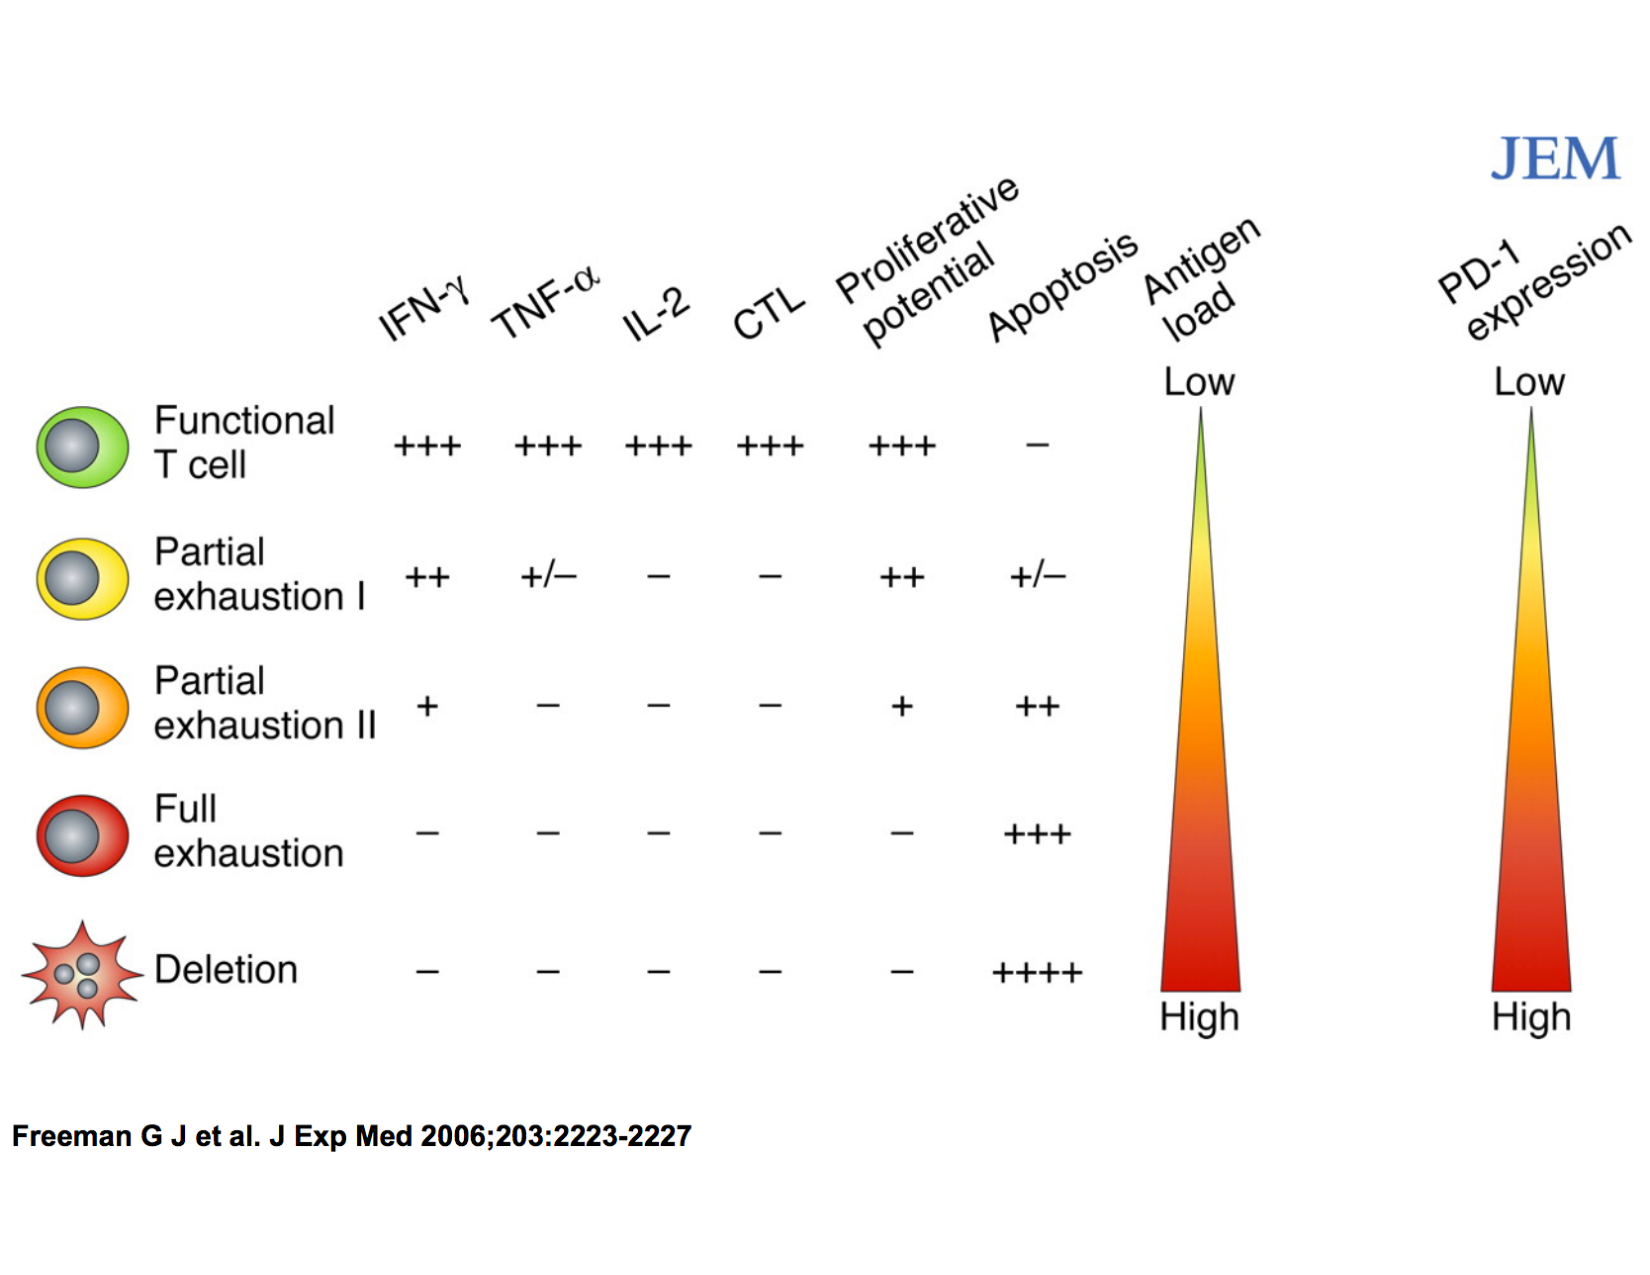
\includegraphics[width=\textwidth]{exhaustion}
\caption{Schematic illustration of factors differentiating active from exhausted T cell populations}
\label{fig01}
\end{figure}

Specifically, this response is meant to prevent an uncontrolled inflammation response that becomes ultimately deleterious to the host. In the case of chronic infection, however, this results in a failure of the host immune system to mount a response to the pathogen.

In the context of viral oncogenesis, we see that, although chronic infection with an oncogenic virus is necessary for carcinogenesis, it is not alone sufficient and must be present in concert with immune dysregulation (immunosuppression or chronic inflammation). Hereby, we see that chronic infection with an oncogenic virus leading to T cell exhaustion fulfills these criteria and provides a favorable environment for carcinogenesis. Indeed, in instances such as this, we may see, for example, viral generation of reactive oxygen species that in turn promotes host cell mutations and can result in tumor formation that is not prevented in the early stages by a robust immune response.

With respect to oncolytic viral therapy, there are numerous physical and immunological barriers to overcome before such a therapy can be truly efficacious and effective. Importantly, these viruses must: (1) be able to evade the host immune response and subsequent opsonization and destruction; (2) replicate exclusively in tumor cells and not systemically throughout the host; (3) must not be capable of inducing disease in the host; and (4) must successfully destroy the tumor.

To achieve high affinity of the oncolytic virus for replication within tumor cells and not systemically throughout the host, the virus may be genetically engineered or, alternately, passaged serially in tumor cells to select for variants that are optimized for replication in such an environment and not in a healthy cellular environment. Additionally, through reverse genetic engineering elements to evade or otherwise prevent viral neutralization by the host immune response may be added to the viral genome. Further, genes or gene segments responsible for pathogenesis may be deleted to render the virus largely safe to the host. Finally, these therapies will often be co-administered with standard-of-care cancer immunotherapeutics to either immunosuppress the host or kill virus-resistant tumor cells and promote tumor-specific immune responses (e.g., via histone deacetylase inhibitors).

\paragraph{6a. Vaccines.} Purely on the basis of the information presented here, I would question the decision to purchase any of the given patents. Specifically, each of these drugs is currently in pre-clinical trial stages, indicating likely that only molecular \textit{in vitro} work has been performed to date. No indication of whether basic toxicity and related pre-clinical data have been yet collected for any of these compounds. Moreover, no indication is here given of the specific molecular mechanisms on which these compounds act. It is impossible from the information given to determine whether any of these compounds has the capability to generate an enduring immune response that is capable of effectively neutralizing HIV upon presentation with live virus.

Approaching this from a financial perspective, I would note that there currently exist 31 independent antiretroviral drugs approved in the United States for the management of HIV-1. Considering this, it becomes not only a question of which of these compounds has the potential to become successfully licensed as an antiretroviral for use in HIV-1 management, but in what ways it would surpass the drugs currently on the market and what incentive there would be for physicians and healthcare providers to prescribe this drug over any other. Certainly, there do not exist or have not been presented any data to indicate that any of these compounds can successfully outcompete the current market offerings, even if they do make it through Phase III clinical trials and are approved for market release in the United States.

Further, what is the benefit of any of these compounds in, by any means, incredibly early stages of development, to something such as adeno-associated virus-expressed eCD4-Ig (a fusion of CD4-Ig and a CCR5-mimetic sulfopeptide) that has shown greater potency than any other HIV-1 broadly neutralizing antibody and that, in a rhesus macaque model, provided long-term immunity to subsequent and repeated challenge with SHIV-AD8?

Even ignoring these factors, would any one of these compounds be effective by itself? or would the vaccination strategy require a prime-boost strategy? If the latter, would, for instance, a combination of the live attenuated vaccine and the virus vectored vaccine be appropriate? Certainly, HIV-1 has a pronounced capability to avoid detection by the host immune system; do we have any evidence to expect that the attenuated virus would function any differently? A similar criticism might be levied against the purified inactivated vaccine: although yes, these can yield production of neutralizing antibodies, will this be the case for HIV-1 and will the immune response to the purified inactivated vaccine be comparable to any subsequent response to challenge with live virus?

A strategy using a DNA vaccine \textit{may} be promising, given that in such strategies the plasmid is taken up by professional antigen-presenting cells which then express the plasmid-encoded genes to generate target antigens. Yet, would this be sufficient for detection of neutralizing antibody-binding sites on the viral envelope that are masked?

Ultimately, until questions such as these are better addressed, I would not feel sufficiently convinced of the merit of any of the proposed compounds to successfully make it to market and become profitable; likewise, I would be unable to recommend the purchase of any of the patents.

\paragraph{6b. Vaccines} Vaccination is a hot-button topic right now; there's no real getting around that. On one side of the argument, you hear cries of individual liberties being violated or of vaccination causing psychiatric disorders. From the pro-vaccination crowd you hear how irresponsible non-vaccination is; how it poses an imminent threat to the health of our society.

If you look at the research, the debate goes to the pro-vaccination crowd: any link between vaccination and autism has been soundly debunked. Although there are risks inherent to vaccines, those risks are all relatively minor and far outweigh, by an large, the risks of a severe case of the disease against which you're vaccination. The argument that mandatory vaccination violates individual liberties is more valid, but certainly we see in many European countries that this mandate is unnecessary for the mainstream adoption of vaccination.

But is any of that really important? If you look at recent statistics, the U.S. has outstandingly high nationwide vaccination rates. The sky isn't falling; the fabric of our society isn't crumbling away. There's a lot of hype but not much substance behind it. There are, however, isolated pockets of low vaccination rates, and though concerning, this by no means rises to the level to which many involved in the vaccination debate elevate it.

What this leads me to ask is whether we are framing this discussion correctly (I would argue that no, we aren't). Specifically, the pro- and anti-vaccination debate is too often little more than ad hominem hurled from each side at the other. Nowhere do we see a legitimate, level-headed discussion about, say, better regulating adjuvants and other compounds included in vaccines that currently do not, under federal law, have to be fully disclosed to the public. Nowhere do we see discussions of when it's appropriate to delay vaccination of your child by 6 months. Nowhere do we see discussion of the relative importance of different vaccines. (Don't want the MMR vaccine? Maybe not a great idea. Choose not to get this year's flu vaccine? Arguably much less pressing.)

Whatever the case, there are legitimate questions to ask regarding vaccination that simply aren't being asked. And that's a problem with our current discourse. Regardless of your position, I'd encourage anyone involved with this debate to take a step back and question how they've been approaching this.

It's not reasonable to expect that we will ever have perfect agreement on which vaccines are appropriate to administer and when, and no, not all of the concerns raised are valid or rational, but neither is that an excuse for vilification. That approach just muddies the waters without addressing the legitimate concerns and questions that many new parents facing a daunting vaccination regiment for their children have.

\paragraph{7. Regulation / Commercialization.} Historically, our regulation of drugs, vaccines, and other therapies has been markedly conservative: devices and drugs are subject to years of rigorous pre-clinical and clinical testing before making it to market, requiring tens to hundreds of millions, or even billions, of dollars in up-front investment. And certainly, we have seen great benefits from this approach: we don't have to look any further than thalidomide and the birth defects it caused throughout Europe for evidence of this.

However, as medical and basic scientific knowledge advances, we see that our regulatory structure has failed utterly to keep pace; it has been unable to keep up with individualized medical treatments, with novel therapeutics that don't fit neatly within the category of `drug' or `device.' And as a result of this, we see that many promising therapies are falling dramatically short of their potential.

For instance, utilizing viruses to treat cancer represents a potentially dramatic leap forward in our ability to manage and even cure the disease and to reduce the economic burden that it places on our country. Yet, if a single virus is developed to combat a single stage of a single type of cancer, what happens when that tumor becomes resistant to the virus? Science might tell us that an easy tweak to the virus is all that was needed to overcome this. But our regulatory structure informs us that a decade of clinical testing and another billion dollars in investment is needed before that therapy can ever make it into the clinic.

What this represents to me is a system that has failed to adapt with the science and that now, instead of protecting patients all-too-often stifles our ability as scientists to help treat them. Accordingly, I would strongly urge you to advocate reform of our current regulatory structure for drugs, devices, and other novel therapeutics. By recognizing therapies like these that do not fit neatly into an established regulatory category, and allowing rapid iterations on these, we can dramatically increase the pace of medical innovation, both at home and as a model the world over.

%%%%%%%%%%%%%%%%%%%%
%% REFERENCES
%%%%%%%%%%%%%%%%%%%%

% \clearpage
% \bibliographystyle{apacite}
% \bibliography{references}

\end{document}